\documentclass[output=paper]{LSP/langsci}
\author{David Kaufman}
\title{Two Siouan languages walk into a Sprachbund}
\abstract{In this paper, I examine two Siouan languages, Biloxi and Ofo, and how they have been influenced by their participation in the Lower Mississippi Valley (LMV) language area, or Sprachbund, which I previously analyzed in-depth in my dissertation. The LMV Sprachbund shows the convergence of eight languages of different language families, including four isolates: Atakapa, Biloxi, Chitimacha, Choctaw-Chickasaw, the Mobilian Trade Language (MTL), Natchez, Ofo, and Tunica, from ca. 500 CE --1700 CE. This Sprachbund involves moderate levels of copying, not only of lexical items but also of grammatical elements. As members of this Sprachbund, Biloxi and Ofo share several phonetic and phonological, morphological, and lexical features with other LMV languages, which are examined here. KEYWORDS: [Siouan, sprachbund, Biloxi, Ofo, convergence area]}
\maketitle

\begin{document}

\section{Introduction}
In this paper, I examine two Siouan languages, Biloxi (ISO 639-3: bll) and Ofo (ISO 639-3: ofo), and how they have been influenced by their participation in the Lower Mississippi Valley (LMV) language area, or \textsc{Sprachbund}\footnote{\emph{Sprachbund} is a German term literally meaning `language union'.} (\citealt[3]{Kaufman2014}). As members of this Sprachbund, Biloxi and Ofo share several phonetic and phonological, morphological, and lexical features with other LMV languages, which are Atakapa, Chitimacha, Choctaw-Chickasaw\footnote{Since Choctaw and Chickasaw are generally mutually comprehensible, I combine them here into one unit.}, Mobilian Trade Language (MTL; also called Mobilian Jargon), Natchez, and Tunica. All of these languages, with the exception of Biloxi and Ofo (Siouan), and Choctaw-Chickasaw and MTL (Muskogean), are isolates with no known living linguistic relatives. 

\begin{figure}
\caption{Lower Mississippi Valley} \label{map}
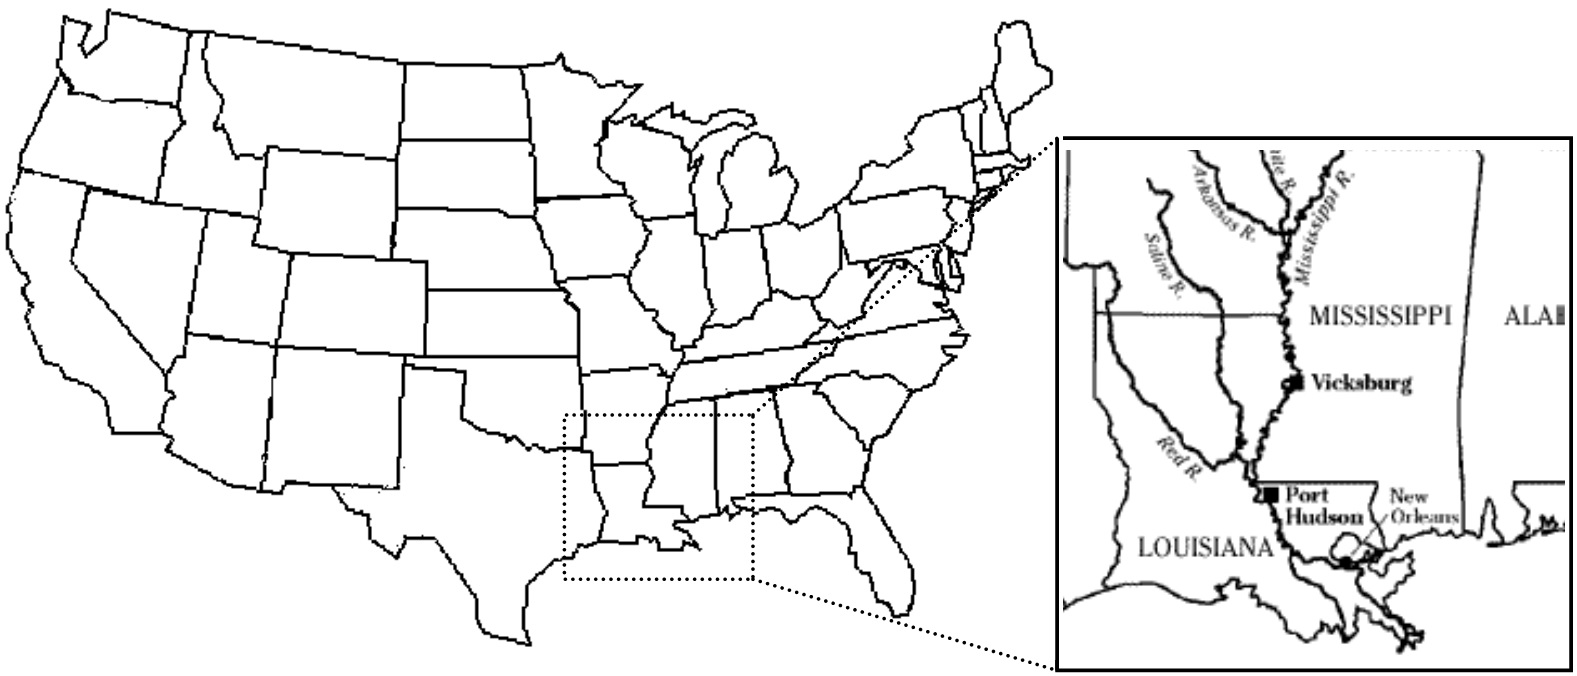
\includegraphics[width=12cm]{figures/Kaufman1}
\end{figure}

I define the Lower Mississippi Valley (LMV) as an area extending from about 260 miles (418 km) west of the Mississippi River eastward to Mobile Bay on the Gulf of Mexico, a total of about 380 miles (612 km), and about 425 miles (684 km) northward from the Gulf of Mexico toward the vicinity of the Tombigbee and Arkansas Rivers, an area encompassing 144,600 square miles (496,600 square km). This area encompasses what is now northern Arkansas, Mississippi, and Alabama, southeastern Oklahoma and eastern Texas over toward central Alabama, and includes all of the modern states of Louisiana and Mississippi; see \figref{map}. My examination of the LMV reveals this region to be a language area on par with the Balkans (Eastern Europe), South Asia (India), the Amazon Basin, and other such Sprachbünde around the world.

Biloxi and Ofo, along with Tutelo, form part of the Ohio Valley, or Southeastern\footnote{I use the term \emph{Southeastern} rather than “Ohio Valley” for this branch of Siouan, since habitation for all members, with the exception of Ofos (Mosopeleas), of this branch in the Ohio Valley is uncertain.}, branch of the Siouan language family. While it is unknown exactly when Biloxis and Ofos reached the LMV, we do have evidence that the Ofos (Mosopeleas) migrated into the LMV in the seventeenth century. Biloxis are harder to pin down, but given the scraps of language data available to us based on toponyms, it is likely that ancestral Biloxis once occupied the southern Appalachian mountain region, probably in the Cumberland Plateau and areas of modern eastern Tennessee near the Tennessee River (see \citealt{Rankin2011} and footnote \ref{waasi}) from where they likely migrated southward to the Gulf coast.\footnote{\label{waasi}Further language evidence, based on toponyms, indicates that the Biloxi word for `salt', \emph{waasi}, may occur in a couple of place names in this region: Ouasioto (\emph{Waasi-oto}?) and Guasile (\emph{Waasi-le}?). The first is the old name for Cumberland Gap, which was indeed situated near a salt-producing mound town (\citealt{Meyer1925}). However, I have no good linguistic explanations for the suffixes \emph{-oto} and \emph{-le} in these names, which do not immediately appear to be Biloxi based on extant data, so that, though intriguing, a definite correlation cannot be made with Biloxis or their ancestors.}

Linguists have long used the Stammbaum (`family tree') model of linguistic ancestral descent, which is usually described with a biological metaphor: the “genetic” origins of languages, which insist on a “single-parent source and its belief that practically all language change resulted from internal causes” (\citealt[7]{Winford2003}). In this case, Proto-Siouan would be the “single-parent source,” while the modern Siouan languages, including Biloxi and Ofo, would be its descendants. However, language change can also arise from external causes through language contact, where similarities arise not through genetic affiliation but through close cultural and linguistic contact. Language areas arise when languages, which may or may not be “genetically” related, come into close contact through such things as trade, alliance, intermarriage, and intergroup gatherings, thereby encouraging “diffusion of linguistic features across geographically adjacent languages” (\citealt[7]{Winford2003}). The LMV was a major hub of trade and contact between many different ethnolinguistic groups, enabling contact among speakers of various languages. 

\section{Internal versus external language developments}

While the bulk of this paper will focus on external, or contact-driven, change, I should mention certain internal developments that make the Southeastern branch of the Siouan language family unique from other Siouan branches. Among the shared phonological innovations of Southeastern Siouan are common Siouan \emph{*š} to Southeastern \emph{č} (e.g., Biloxi \emph{čǫki}, Ofo \emph{ačǫki}, Tutelo \emph{chǫ:ki} `dog' \footnote{Biloxi terms are based on \citet{DorseySwanton1912}, Ofo terms on Rankin’s reanalysis \citeyearpar{Rankin2002} of \citet{DorseySwanton1912}, and Tutelo terms on \citet{Oliverio1996}.}) and the merger of glottalized and non-glottalized stops (\citealt{Rankin2011}). Shared lexical innovations include innovative terms for `road' (Biloxi \emph{natkhohi}, Ofo \emph{nakhó•hi}, Tutelo \emph{hątkóx}; `prairie' (Biloxi \emph{takohǫ}, Ofo \emph{akhó•hi}, Tutelo \emph{lata:hkoi}, \emph{oni:i}); and `squirrel' (Biloxi \emph{ąsaki}, Ofo \emph{tó•staki}, Tutelo \emph{hista:xkai}); and fusion of the terms for `grizzly' and `black bear' (Biloxi \emph{ǫti}, Ofo \emph{ųthi}, Tutelo \emph{hamǫ:thi}, \emph{mǫ:ti}) (\citealt{Rankin2011}). Shared morphosyntactic innovations include the auxiliation of \emph{yukê} `be (\textsc{pl})' and `durative aspect', collapse of the `here/there,' or `home base / apogee' (\citealt[125]{Cumberland2005}), distinction in verbs of arrival, collapse of active/stative argument marking, and split negation (\citealt{Cumberland2005}). These innovations are internal developments that likely occurred before the Biloxi and Ofo migrations into the LMV and the contact-related developments that happened after that.

External, as opposed to internal, language developments arise through languages coming into contact with each other, usually over an extended period of time. The depth of contact between two or more languages can generally tell us how long those groups were in contact. Lexical and phonetic features, which are easily recognizable surface features in languages, can be borrowed between groups with minimal contact and are thus weighted lower in determining the overall strength of a Sprachbund (\citealt{Kaufman2014}). Morphological features, which are more deeply embedded in the grammatical structure of languages, are more difficult to borrow and require more intimate contact to develop. Thus, morphological features are weighted more highly (\citealt{Kaufman2014}).

For this paper, I address only those features I weighted more highly in \citet{Kaufman2014} -- those given a score of 2 (the features most indicative of an LMV Sprachbund), and only if they occur in the LMV Siouan languages\footnote{In \citet{Kaufman2014}, I weighted features on a tripartite scale of 0, 1, and 2. A score of 0 indicates that the feature in question does not exist in the area I delimited as the LMV. A score of 1 indicates that the feature exists in the area but is so common crosslinguistically that its presence in the LMV is not distinctive and thus not deemed relevant to supporting the LMV as a Sprachbund. A score of 2, the highest weighting, indicates that the feature is either geographically limited to the LMV and its immediate periphery, or is so unusual crosslinguistically as to be especially relevant in supporting the LMV as a Sprachbund (\citealt{Kaufman2014}).}. Phonetic and phonological features discussed are: (1) nasalized vowels; (2) voiceless labiodental fricative /f/; (3) alternation of /i/ and /u/; and (4) alternation of word initial /h/ \textasciitilde{} /Ø/. Morphological features discussed are: (1) focus and topic (discourse) marking, (2) valence-reducing prefix, (3) positional verb auxiliaries and (4) verb number suppletion. 

I will then discuss lexical items that appear to have been shared among LMV languages, particularly those involving Biloxi and Ofo. Although lexical features were scored differently from phonetic/phonological and morphosyntactic features (see \citealt{Kaufman2014}) and are weighted less overall, it has been long noted that certain lexical items appear broadly diffused in the region. 

\section{Phonetic and phonological features}

\subsection{Nasalized vowels}

Nasalized vowels are a feature of Siouan and Muskogean languages. All Siouan languages, with the exception of Hidatsa and Crow, have vowel nasalization, including Biloxi and Ofo. Nasal vowels also occur in the LMV languages Atakapa, Choctaw-Chickasaw, MTL, and Natchez. In Natchez, however, nasal vowels occur only in phrase- or sentence-final position and are thought to be based on underlying final /n/, which acts as a type of declarative marker (Geoffrey Kimball 2013, p.c.). Vowel nasalization in Atakapa is at times uncertain, perhaps being an allophone of the phoneme /ŋ/. Vowel nasalization in Atakapa and Natchez may be due to contact with LMV Siouan and Muskogean languages, although such nasalization may also be due to internal impetus.

\subsection{Voiceless labiodental fricative /f/}

Only one Siouan language, Ofo, has this phoneme, although all Muskogean languages, including MTL, have it. Haas postulated Muskogean /f/ as the modern reflex of Proto-Muskogean /xw/ (\citeyear[36]{Haas1969}). Biloxi may have had at least a dialectal reflex of /xw/ pronounced as /f/, as evidenced by Mrs. Jackson’s pronunciation of \emph{nixuxwi} (\emph{nišofeˀ}) `ear' (\citealt[79]{HaasSwadesh1968}), a pronunciation that correlates with the probable change of Proto-Muskogean /xw/ to /f/. (It is unclear whether this was a dialectal feature of Biloxi at the time data were elicited or whether this was an idiosyncratic pronunciation based on possible personal influence of Choctaw-Chickasaw.). This phoneme is also found in Atakapa, though rare and usually in word-final position, and may be due to internal impetus such as through fricativization of word-final labiodental velar /w/.

\subsection{Alternation of /i/ and /u/}
	
The alternation of /i/ and /u/ occurs in Biloxi, Natchez, and Tunica. This alternation appears to be a feature of Siouan languages, particularly of Biloxi but also of Dhegiha Siouan languages. The transition of /u/ to /i/ in Siouan is most apparent in Kansa (Kaw), wherein /u/ is pronounced like German \emph{ü} (/y/), apparently midway in transition between /u/ and /i/. (\citealt{DorseySwanton1912} also occasionally note the phoneme /y/ in Biloxi pronunciation, though it was apparently infrequent.) Examples include Biloxi \emph{ci} and \emph{cu} `put, place, plant'; Natchez \emph{išuš} and \emph{ušuš} `back'; and Tunica \emph{tahišini} \textasciitilde{} \emph{tahišuni} `sieve';  \emph{hiši} \textasciitilde{} \emph{hišu} `sift'.

This feature is crosslinguistically rare and is not likely a genetic or internally developed feature. It is likely that this feature’s occurrence in Natchez and Tunica arose through contact with Siouan languages, although it could also be the result of vowel harmony. 

\subsection{Alternation of word initial /h/ \textasciitilde{} Ø}

The alternation of word initial /h/ \textasciitilde{} Ø (zero marking) is a feature of the LMV area that occurs in Biloxi as well as in Atakapa and MTL. Examples include Atakapa \emph{hipa} \textasciitilde{} \emph{ipa} `husband' (\citealt[42]{GatschetSwanton1932}), \emph{hikat} \textasciitilde{} \emph{ikat} `foot' (\citealt[40]{GatschetSwanton1932}), \emph{himatol} \textasciitilde{} \emph{imatol} `four' (\citealt[41]{GatschetSwanton1932}) and \emph{huket} \textasciitilde{} \emph{uket} `mother' (\citealt[46]{GatschetSwanton1932}); Biloxi \emph{hane} \textasciitilde{} \emph{ane} `find', \emph{hamihi} \textasciitilde{} \emph{amihi} `heat' and \emph{hasne} \textasciitilde{} \emph{asne} `thief' (\citealt[3]{DorseySwanton1912}); and MTL \emph{hat(t)ak} \textasciitilde{} \emph{atak} `man' (\citealt[88]{Crawford1978}; \citealt[295]{Drechsel1996}) and \emph{hoyba} \textasciitilde{} \emph{oyba} `rain' (\citealt[306]{Drechsel1996}). This feature appears to be a Siouan-language-internal development, since “glottal stop is often inserted before word-initial vowels in Siouan sentences as a Grenzsignal — a boundary marker — so it is possible that the Biloxi initial \emph{h-} that comes and goes in these words is the local reflex of [ʔ]”  (\citealt[3]{Rankin2011}). Regarding MTL, the alternation appears “to be instances of an \emph{h-} that was present etymologically in Western Muskogean that was lost among certain users of Mobilian” (\citealt[3]{Rankin2011}). Since the change from [ʔ] to \emph{h-} appears to be an internal Siouan development, it is possible that this feature was copied from Siouan (Biloxi) into Atakapa and MTL. 

\section{Morphological features}

The ranking of morphological features is a bit trickier than for phonetic and phonological features, since data on morphological features for languages in and around the LMV are often lacking in specific features. For example, MTL totals very low on the morphological-features scale simply because the language, typical of pidgins, is largely isolating and contains few morphological features. Ofo also scores low, simply because extant data on the language is scanty, not because it did not participate more fully in the LMV language area.

	Morphological features that have been determined most relevant in analyzing the LMV as a Sprachbund (\citealt[3]{Kaufman2014}) are:

\begin{enumerate}
\item{Focus and topic marking.}
\item{Valence-reducing prefix.}
\item{Positional verb auxiliaries.}
\item{Verbal number suppletion.}
\end{enumerate}
 
These features have been determined most relevant in the analysis of an LMV Sprachbund partly because of their limited overall distribution beyond the LMV and their relative rarity among the world’s languages. Such limited distribution indicates a comparatively confined area probably once having a high volume of ongoing contact.

\subsection{Discourse marking}

Pragmatic or discursive affixation such as focality and topicality marking is fairly common among Native American languages. I use the term \textsc{discourse-marking} to include speaker-centered emphatic marking, often labeled \emph{focus}, \emph{topic} and \emph{assertion}, as well as evidentiality and reference tracking. These markers, in each language in which they occur, are discussed below.

\subsubsection{Focus}
	
I use the term \textsc{focus} to refer to new information (what Prague School linguists call “rheme”) (\citealt[271]{Payne1997}).\todo{Reference missing from author's original.} LMV focus-marking suffixes can occur on both nouns and verbs.

	Biloxi, along with Atakapa, Chitimacha, Choctaw-Chickasaw, and Natchez, has focus-marking suffixation. Atakapa and Chitimacha appear to share a focus-marking suffix \emph{-š} while Choctaw-Chickasaw and Natchez appear to share the suffix \emph{-ook}. Unfortunately, focus and topic marking cannot be discerned in Ofo from extant data.

In Biloxi, the marker \emph{-di} is often suffixed to nouns in texts, particularly with nouns newly introduced into the narrative or discourse (\citealt[3]{Kaufman2011}). The suffix \emph{-di} descends directly from Proto-Siouan \emph{*-ri}, a focus marker also found in Hidatsa and Mandan (\citealt[3]{Boyle2007}, p.c.). This suffix is sometimes used at first mention when objects or characters are first introduced into a story, thus signaling new information. 

\ea\label{possumpond}
\gll 	Skakana-\textbf{di} ewite-xti eyąhi yuhi yohi-y\k{a}. \\
	Ancient.of.Opossums-\textsc{foc} early-\textsc{intens} \textsc{3sg}-arrive \textsc{3sg}-think pond-\textsc{top}\\
\glt `The Ancient of Opossums thought he would reach a certain pond very early in the morning.' (\citealt[26]{DorseySwanton1912})
\z

\ea
\gll	Ąyaa-\textbf{di} wax ni yukê \\
	person-\textsc{foc} hunt walk \textsc{move}\\
\glt `Some people were hunting ...' (\citealt[65]{DorseySwanton1912})
\z

\subsubsection{Topic}

I use the term \textsc{topic} to refer to old, previously mentioned, or known information (what Prague School linguists call “theme”) (\citealt[271]{Payne1997}).\todo{Reference missing from author's original.} Biloxi and Choctaw-Chickasaw have suffixes that serve as types of definite article, indicating previous mention. Biloxi \emph{-yą} is a form of definite article that tends to occur most frequently when the noun to which it is suffixed has already been introduced into a story, thus marking old or already given information, as the following examples show: 

\ea
\gll	Ątatka-\textbf{yą } khu-ni 	 ǫǫni e-tu 	 xa.\\ 
child-\textsc{top} 3.give-\textsc{neg} \textsc{pst} 	 3.say-\textsc{pl} always \\
\glt `Always she did not give him the child.' (`She never gave him the child'?) (\citealt[43]{DorseySwanton2012})
\z

\ea
\gll	“Yamą na,” 	 e-di 	 ąyaa-xohi-\textbf{yą}\\
	\hspace{.6em}no 	\textsc{decl.m} 3sg.say-\textsc{asrt} person-old-\textsc{top} \\
\glt ```No,'' the old woman said.' (\citealt[67]{DorseySwanton2012})
\z

In the above examples, `child' and `old woman' were previously mentioned in the discourse.\footnote{In example \ref{possumpond} above, \emph{-yą} appears on \emph{yohi} `pond', though the pond is not previously mentioned in the text. However, since this certain pond is already known to the Ancient of Opossums, it seems to be treated as previous knowledge, or a previously known location that can take the definite article marker.}

	The Choctaw-Chickasaw suffix \emph{-aaš} indicates previous mention, in essence acting as a type of definite article:

\ea
\gll	Hattak-Ø-\textbf{aaš}-at čaaha-h.\\
	man-\textsc{cop-prev-nom} tall-\textsc{tns} \\
\glt `The previously mentioned man is tall.' 
(\citealt[89]{Broadwell2006})
\z

\subsubsection{Assertive marking}

Biloxi, along with Atakapa, Chitimacha, and Natchez, has assertive markers, with which a speaker may choose to add particular emphasis or immediacy to a verb. 

	We have seen the Biloxi focus marker \emph{-di} attached to nouns, but the suffix \emph{-di} also attaches to verbs. With verbs, \emph{-di} shows more emphasis or immediacy and has been glossed as an “assertive” marker (\citealt[3]{Kaufman2011}), as the following examples demonstrate:

\ea
\gll	Sǫǫnitǫǫni-k ǫha ąyaa ǫǫni ustax kanê-\textbf{di} \\
	tar-\textsc{acc}  with man make stand.up \textsc{evid-asrt}\\
\glt `He made a tar baby [person] and stood it up there.' (\citealt[13]{DorseySwanton1912})
\z

\ea
\gll	Kąkǫǫni dǫhi tê dê-\textbf{di} ê-tu-xa\\
	trap 	 see want go-\textsc{asrt} they-say-always\\
\glt `They say that he departed, as he wished to see the trap.' (\citealt[184]{DorseySwanton1912})
\z

\subsection{Valence-reducing prefix}

All languages have operations that adjust the relationship of semantic roles and grammatical relations in languages, using a range of structures for accomplishing this (\citealt[169]{Payne1997}).\todo{Reference missing from author's original.} In the LMV, a preverb or prefix is used as a valence-reducing operation. Atakapa, Biloxi, Chitimacha, Choctaw-Chickasaw, Natchez, and Ofo all have valence-reducing prefixation. 	

	Siouan languages have a prefix \emph{wa-} (reduced to \emph{a-} in Biloxi and Ofo\footnote{Biloxi and Ofo normally lose word-initial labial resonants, or most reflexes of \emph{*w}, \emph{*m}, and \emph{*W} (\citealt[19]{Rankin2002}).}), whose actual translation is murky, though it often can be translated as `thing' or `something' (i.e., an indefinite object prefix) and acts as a type of valence reducer (\citealt[3]{Rankin2013}, p.c.):\todo{no 2013 paper by Rankin in bib}

\ea
\gll	\textbf{a}-duska\\
		thing-bite\\
\glt	 `rat' (\citealt[186]{DorseySwanton1912})
\z

	In Atakapa, the valence-reducing prefix is \emph{šok-}:

\ea
\gll	\textbf{šok}-koi\\
		\textsc{indf.obj}-speak \\

\glt	`chief' (`speaking things') (\citealt[9]{GatschetSwanton1932})
\z

The Chitimacha valence-reducing preverb is \emph{ni}:

\ea
\gll	\textbf{ni} 	katš hamtši:k \\
	thing fortune having\\

\glt `having (good) luck' (Hieber 2013, p.c.)\todo{Reference missing from author's original.}
\z

	The Choctaw valence-reducing prefix is \emph{naa-} or \emph{nąn-}:
	
\ea\label{hunterprey}
\gll	\textbf{naa}-hóoyo-ʹ~\\
		\textsc{indf.obj(subj)}-hunt-\textsc{nzr}\\
\glt	`hunter' or `prey' (\citealt[53]{Broadwell2006})
\z

Example \ref{hunterprey} demonstrates that Choctaw \emph{nan-} or \emph{naa-} can be ambivalent, since the preverb \emph{naa-} can represent either the actor (hunter) or the patient (prey) (\citealt[53]{Broadwell2006}). The Western Muskogean prefixes \emph{nąn-} and \emph{naa-} likely derive from the word \emph{nąta} `what, something, someone.'
 
	The Natchez valence-reducing prefix is \emph{kin-}:
	
\ea	nokkinhantawąą\\
\gll		nok-\textbf{kin}-han-ta-w-aa-n\\
		\textsc{pvb-indf.obj}-make-\textsc{1sg-aux-inc-phr.trm}\\
\glt	`I can work.' (\citealt[405]{Kimball2005})
\z

\subsection{Positional verb auxiliaries}

Classificatory verbs of the LMV signal position classification of noun referents: \textsc{sit}, \textsc{stand}, \textsc{lie}, and \textsc{move}, which occur as markers of continuative aspect in most if not all of the Siouan languages (\citealt[203]{Rankin2004}).\todo{2004 a or b?} Positional verbs have been grammaticized in the Siouan languages as continuative aspect markers and proximal demonstrative determiners (\citealt[116]{Mithun1999}). Biloxi and Ofo, along with Atakapa, Chitimacha, Choctaw, and Tunica, all use positionals in a similar manner, indicating possible borrowing between them. 

\ea
\settowidth\jamwidth{(Choctaw-Chickasaw)}
\gll	Nihǫ 	ani 	dêxtowê \textbf{nê}.\\
		cup water full  \textsc{stand}\\ \jambox{(Biloxi)}
\glt	`The cup is full of water.' (\citealt[166]{DorseySwanton1912})
\z
		
\ea
\settowidth\jamwidth{(Choctaw-Chickasaw)}
\gll	b-ashě \textbf{nąki}\\
		1-sit \textsc{sit}\\ \jambox{(Ofo)}
\glt	`I am sitting down.' (\citealt[20]{Rankin2002})
\z

Positional verbs are also used for continuative aspect in other LMV languages, as these examples show:

\ea
\settowidth\jamwidth{(Choctaw-Chickasaw)}
\gll	keu kam-š-kin-\textbf{tu}\\
		sit protrusion-\textsc{def-loc-stand}\\ \jambox{(Atakapa)}
\glt `I am [seated] paddling.' (\citealt[61]{GatschetSwanton1932}; \citealt[27]{Watkins1976})
\z

\ea	
\settowidth\jamwidth{(Choctaw-Chickasaw)}
wekt kas tuhjyi:kʔ peʔanki \jambox{(Chitimacha)}
\gll		we-t-k 	 kas 	 tuhjte-:ikʔ 	 \textbf{pe}-ʔe-nk-i\\
		\textsc{dem-refl-loc} back	  stoop.down-\textsc{prtp} be(horizontal)-\textsc{3sg-loc-nzr}\\
\glt	`when he had stooped down' (Swadesh, unpublished notes)
\z

\ea
\settowidth\jamwidth{(Choctaw-Chickasaw)}
\gll	Bill-at ma \textbf{binįli}\\
	 \textsc{subj} there sit.\textsc{anim}\\ \jambox{(Choctaw-Chickasaw)}
\glt `Bill is (sitting) over there.' (\citealt[21]{Watkins1976})
\z
		
\ea	
\settowidth\jamwidth{(Choctaw-Chickasaw)} 
yaˑ potkop kaʔašup kaʔepeˑnakiyakuˑš\footnotemark \jambox{(Natchez)}
\gll		yaˑ potkop kaʔašup-Ø kaˑ-\textbf{ʔepeˑ}-na-ki-ya-kuˑš\\
		that mountain blue-\textsc{abs} \textsc{pvb}-lie-\textsc{3pl-aux-art-all}\\
\glt	`(where) that blue mountain is (lying)' (\citealt[438]{Kimball2005})
\z

\ea
\settowidth\jamwidth{(Choctaw-Chickasaw)}
\gll	t-uruna-tʔe-ku 	\textbf{ʔuna}\\
 \textsc{def}-frog-large-\textsc{m.sg} sit\\ \jambox{(Tunica)}
\glt `There is the (sitting) bullfrog.' (\citealt[26]{Watkins1976})
\z

In many languages of the world the same lexical item can express both actual physical stance and can be used as an auxiliary, as is demonstrated in the Chitimacha, Choctaw-Chickasaw, Natchez, and Tunica examples above. In Biloxi and Ofo, however, physical stance and locative-existential predicates/verbal auxiliaries generally form two different sets of lexemes. The stance verbs used as independent verbs in Biloxi are \emph{toho} `lie', \emph{xêhê} `sit', \emph{sįhį} `stand', and \emph{hine} and \emph{ni} `move'. In Ofo the independent verbs are \emph{čáftu} `lie', \emph{áshĕ} `sit', and \emph{askho(le)} `stand' (there is no data for `move' in Ofo). Their grammaticized auxiliary counterparts are \emph{mąki} `lie' and \emph{nąki} `sit' in both Biloxi and Ofo, while \emph{nê} `stand' and \emph{ąde} and \emph{hine} `move' occur in Biloxi but are unattested in Ofo. The Biloxi form \emph{hine} is used for both singular and plural while \emph{ąde} has a suppletive plural form, \emph{yukê}. \emph{Ąde} is used for general movement and running while \emph{hine} is for walking only (\citealt[3]{Kaufman2013}). 

These verbs form a discrete set of auxiliary verbs that often no longer specify actual physical position or movement but, rather, are used to express nuanced aspectual meanings. Biloxi \emph{mąki}, \emph{nąki}, and \emph{nê} are used for both animates and inanimates, while \emph{ąde} and \emph{hine} are confined to use only with animates. \emph{Mąki}, \emph{nąki}, and \emph{nê} share a common plural form \emph{(h)amąki}, apparently a form of \emph{mąki} `lie'. 
 
\subsection{Verbal number suppletion}

	For this section, the definition of suppletion includes cases that satisfy either of the following criteria: (1) exceptions to very productive derivational patterns, and (2) exceptions to established agreement patterns (\citealt[3]{Veselinova2003}). The verbal suppletion treated here relates to nominal arguments of the verb, where the verb agrees with its arguments. All languages of the LMV, except MTL and Natchez, have verbal number suppletion in relation to nominal arguments. This feature is further limited in the region by being primarily used in relation to the positional auxiliaries \textsc{stand}, \textsc{sit}, \textsc{lie}, \textsc{move} (see above). In Tunica, only these auxiliary verbs show suppletion, while other verbs in the language do not (\citealt[40]{Haas1946}). While not displaying direct borrowing of the suppletive terms between the languages, the fact that verbal number suppletion occurs primarily or only in positional auxiliaries makes this a distinguishing feature of the LMV. While the suppletive verb forms may be unique to each language, the underlying pattern of such deviating forms across LMV positional auxiliaries would seem to indicate a deeper-level pattern influence among multilingual speakers of this Sprachbund.

	Verbal number suppletion in each language is shown below:

\begin{table}
\caption{Biloxi (\citealt[3]{DorseySwanton1912})}
\begin{tabularx}{.5\textwidth}{XXX}
\lsptoprule
& singular & plural \\
\midrule
\textsc{stand} & nê & \\
\textsc{sit} & nąki & (h)amąki \\
 \textsc{lie} & mąki & \\ 
 \textsc{moving} & ąde & yukê \\
 \lspbottomrule
\end{tabularx}
\end{table}

\begin{table}
\caption{Atakapa (\citealt[3]{GatschetSwanton1932})}
\begin{tabularx}{.5\textwidth}{XXX }
\lsptoprule
& singular & plural \\
\midrule
\textsc{stand} & to/tu \emph{or} ta & tsot \\
\textsc{sit} & ke & nul \\
\textsc{lie} & tixt & yoxt \\
\lspbottomrule
\end{tabularx} 
\end{table}

Chitimacha, like Biloxi, neutralizes the singular auxiliary forms to a single plural form, \emph{na(h)}.

\begin{table}
\caption{Chitimacha (\citealt[32]{Swadesh1939})}
\begin{tabularx}{.5\textwidth}{ XXX}
\lsptoprule
& singular & plural \\
\midrule
\textsc{stand} & ci(h) &  \\
\textsc{sit} & hi(h) & na(h) \\
 \textsc{lie} & pe(h) &  \\
\lspbottomrule
\end{tabularx}
\end{table}

Choctaw-Chickasaw has both animate and inanimate forms for \textsc{sit}.

\begin{table}
\caption{Choctaw (\citealt[3]{Broadwell2006})}
\begin{tabularx}{.75\textwidth}{lXXX}
\lsptoprule
 & singular & dual & plural \\
\midrule
\textsc{stand} & hikiya\footnotemark & hiili & (hi)yoh- \\
\textsc{sit (anim.)} & binili & chiiya & binoh- \\
\textsc{sit (inanim.)} & talaya & taloha & taloh- \\
 \textsc{lie} & ittola & kaha & kah- \\
\lspbottomrule
\end{tabularx} 
\end{table}

In Tunica, suppletion is “a process not used by any other word-class of the language” (\citealt[40]{Haas1946}). Thus, Tunica suppletion appears to be a borrowed feature from contact with other LMV languages.

\begin{table}
\caption{Tunica (\citealt[40]{Haas1946})}
\begin{tabularx}{.75\textwidth}{XXXX}
\lsptoprule
&  {singular} &  {dual} &  {plural} \\
\midrule
 \textsc{stand} & kali\footnotemark & ? & ? \\
\textsc{sit} & ˀuna & ˀunana & ˀukˀɛra \\
\textsc{lie} & ˀura & ˀurana & naˀara \\
\lspbottomrule
\end{tabularx} 
\end{table}

	It should be noted that Dhegiha Siouan languages, such as Kanza (Kaw), also show some suppletion in positional verbs (e.g. Kaw \emph{yįkhé} `sitting animate/inanimate singular object' and \emph{yąkhá} `sitting animate plural object)'. Whether this is due to contact between Dhegiha Siouan and LMV languages is debatable and remains a possibility to be further studied. The Dhegiha Siouan language Quapaw, for example, was on the LMV periphery.

Unfortunately, in Ofo, only the positional forms \emph{mąki} and \emph{nąki} are attested, so determination of verbal number suppletion is not possible.

\section{Lexical features}

	Lexical borrowing, due to the easy surface-level recognition of lexical items, is considered less important for establishing a Sprachbund. Word borrowings operate according to a certain set of probabilities. Languages are more likely to borrow nouns than verbs (\citealt[231]{Tadmoretal2010}). Adjectives and adverbs are almost as hard to borrow as verbs, and words with grammatical meanings (function words) are harder to borrow than verbs (\citealt[231]{Tadmoretal2010}). Basic vocabulary is borrowed before structure and is indicative of more intense contact, while non-basic vocabulary is easiest to borrow (\citealt[69]{Thomason2001}) and gets borrowed under conditions of even casual contact (\citealt[231]{Tadmoretal2010}). Intensity of contact is, however, “a vague concept, and it cannot be made much more precise because it interacts with speakers’ attitudes as well as with more easily specified factors, such as the level of fluency of the borrowers and the proportion of borrowing-language speakers who are fully bilingual in the source language” (\citealt[231]{Tadmoretal2010}). 

\subsection{Basic vocabulary}

	The concept of basic vocabulary is important to the analysis of lexical borrowings. Several lists have been created to reflect basic concepts that are considered to be universal and culturally independent, such as basic kinship (e.g., \emph{mother}, \emph{father}), general animal terms (e.g., \emph{fish}, \emph{bird}), and basic verbs (e.g., \emph{make}, \emph{go}). The stability of the resulting list of “universal” vocabulary has been brought into question, however, and multiple lists of basic vocabulary have been published. The first was the Swadesh list of 100 basic words.

	The Swadesh list was assembled by the linguist Morris \citet{Swadesh1971}. Swadesh “determined a priori what constituted basic vocabulary based on his intuitions, and then proceeded to refine his list by trial and error” (\citealt[230]{Tadmoretal2010}). A newer list, which I used in analyzing LMV lexical items, is the Leipzig-Jakarta (L-J) 100-word list (2009)\todo{Reference missing from author's original.}. This list (see \tabref{LJ100}) is based on systematic empirical data from 40 different languages. An advantage of the Leipzig-Jakarta list is that it ``has a strong empirical foundation and is thus a more reliable tool for scientific purposes” (\citealt[230]{Tadmoretal2010}). However, as with acceptance of any word list, things are not always perfect and certain questions remain unaddressed, such as why \emph{black} is considered a basic color but not \emph{white}.

\todo{Reference missing from author's original.}
\begin{table}
\caption{Leipzig-Jakarta (2009) list of 100 basic words} \label{LJ100}
\begin{tabular}{llll}    
\lsptoprule                                                                     
 ant                     &    eye                     &       leg/foot         &    small  \\
 arm/hand                &    to fall                 &       liver           &      smoke     \\
 ash                     &    far                     &       long            &     soil      \\
 back                    &    fire                    &       louse           &     to stand  \\
 big                     &    fish                    &       mouth           &     star         \\
 bird                    &    flesh/meat              &       name            &     stone/rock\\
 to bite                 &    fly                     &       navel           &     to suck\\
 bitter                  &    to give                 &       neck            &     sweet \\
 black                   &    to go                   &       new             &     tail \\
 blood                   &    good                    &       night           &     to take\\
 to blow                 &    hair                    &       nose            &     thick \\
 bone                    &    hard                    &       not             &     thigh \\
 breast                  &    he/she/it/him           &       old             &     this \\
 to burn (intrans)       &    to hear                 &         one            &      to tie\\
 to carry                &    heavy                   &       rain            &     tongue \\
 child (recip of parent) &     to hide                &         red           &      tooth\\
 to come                 &      to hit/to beat        &         root          &      water\\
 to crush/to grind       &     horn                   &         rope          &      what?\\
 to cry/to weep          &      house                 &         to run        &      who? \\
 to do/to make           &      I/me                  &         salt          &      wide \\
 dog                     &      in                    &         sand          &      wind \\
 drink                   &      knee                  &         to say        &      wing \\
 ear                     &      to know               &         to see        &      wood \\
 to eat                  &      to laugh              &         shade/shadow  &      yesterday\\
  egg                    &     leaf                   &          skin/hide    &     you (sg) \\
       \lspbottomrule
\end{tabular}                                                                 
\end{table}

\subsection{Semantic classes of borrowings}
	
	The number of borrowings between LMV languages can tell us something about the prior location and migration patterns of LMV groups. For example, the sheer volume of borrowings between Atakapa and Biloxi suggests that these languages were heavily in contact at one time. This seems extraordinary given the post-contact geographic locations of these groups, being on opposite sides of the Mississippi River. It is also notable that there are fewer borrowings between Chitimacha and Biloxi than between Atakapa and Biloxi, even though the Chitimachas, at least given their post-contact location, were in between. This could indicate, however, that Atakapas and Biloxis were geographically much closer to each other at one time. Biloxis may once have been located west of the Mississippi River before migrating eastward to the Pascagoula River region along the Gulf of Mexico where they encountered the French in 1699.

	\tabref{LMVloans} is a list of LMV borrowings by semantic category (L-J basic vocabulary in \textbf{bold}): 

\begin{table}
\caption{LMV borrowings by semantic category} \label{LMVloans}
\begin{tabularx}{\textwidth}{llX}
\lsptoprule
Agricultural & (2) & seed, turn (soil?) \\
Body parts & (9) & anus/back, \textbf{arm/hand}, belly, \textbf{breast}, elbow, face, \textbf{knee},  \textbf{mouth}, \textbf{tooth}  \\
Botanical & (9) & berry, cedar, corn, cotton, cypress, oak, peach, pepper, pumpkin/turnip  \\ 
Color & (2) & black, \textbf{white} \\
Drink & (1) & \textbf{water} \\
Food & (2) & tortilla, bread \\
Kin & (1) & brother \\
Transport & (1) & canoe \\
Weapon & (1) & bow \\
Zoological & (19) & bee, \textbf{bird}, bison / buffalo, blackbird, bullfrog, buzzard, cow/calf, crane, deer, \textbf{dog}, duck, \textbf{fish}, flying squirrel,   raccoon, robin, skunk, snake, wildcat, woodpecker \\
\lspbottomrule
\end{tabularx}
\end{table}

Several basic words appear to have been shared between Biloxi, Ofo, and other LMV languages; see \tabref{sharedvocab}: 

\begin{table}
\caption{Shared basic vocabulary} \label{sharedvocab}
\begin{tabularx}{\textwidth}{ llllllX }
\lsptoprule 
& Atakapa & Biloxi & Chitimacha & Natchez & Ofo & Tunica\\ 
\midrule
 hear & nak & naxe & & & & \\
laugh & hayu & xahaye & & & &
\\ blow & pun & po & puuh(te) & puuh-hoo’iš & &
\\ cord/ & & įką & & & & yúnka
\\ rope & & & & & &
\\ cry & & wahe & & & & wáha
\\ knee & timak & cinąki & & & & cina(hki)
\\ mouth & & ihi & i  `tooth' & ihi & ihi &
\\ wind & & xux(we) & howi & & & húri 
\\ \lspbottomrule
\end{tabularx}
\end{table}

\subsection{Widespread lexical borrowings in the LMV and Southeast}

	Certain nouns, and at least three verbs, are fairly widespread throughout the LMV and Southeast in their diffusion: those for `bison/buffalo', `bullfrog', `cut', `deer', `goose', `metal', `robin', `split', `town', `turn', `water', and `woodpecker'. 

\ea {`Bison / buffalo': Similar terms for `bison / buffalo' are of particularly widespread diffusion, ranging from Caddoan in the western Plains to Catawba near the eastern seaboard, including in the LMV: Bi. \emph{yinisa}, \emph{yanasa}, Choc.-Chic. \emph{yanaš}, MTL. \emph{yanaš}, Nat. \emph{yanašah}, and Tun. \emph{yanši}, \emph{yanškaši}. The Ofo term \emph{naf} `cow' is likely also derived from this widespread `bison' term. While the source of the borrowing is unknown, \citet[166]{Taylor1976b} suggested the possibility of its origin in an Athabaskan language. I concur with him that the Apache \emph{iyaná ɬa’} (with loss of the initial \emph{i} and the second element being the enclitic for indefinite determiner) could indeed be the source of copying. Apaches were a Plains group who may have been in contact on a regular basis with buffalo hunting parties of other groups from the LMV and Southeast and were probably also involved in the buffalo fur trade. Totonac has the word \emph{tiyaná} for `ox,' raising the possibility of borrowing between this Mexican Gulf coastal language and the LMV for this similar bovine perhaps through Mobile Bay.}
\z

\ea {`Bullfrog': Similar terms for `bullfrog' occur in At. \emph{anenui}, Bi. \emph{kǫninuhi}, MTL. \emph{hanono}, Nat. \emph{hánanai}, and Tun. \emph{uruna(te)}. The source language of this borrowing is unknown.}
\z

\ea {`Cut': Similar terms for `cut' occur in At. \emph{kets} or \emph{kuts}, Bi. \emph{kutsi}, Nat. \emph{keš}, and Tun. \emph{kušu}. The Plains languages Comanche, Tonkawa, and possibly Caddoan have terms similar to the LMV form. The source language of the borrowing is unknown.}
\z

\ea {`Deer': Similar terms for `deer' appear to have been borrowed in the LMV as well as in the Plains periphery. The Proto-Siouan form is \emph{*wi-htáa}, indicating possible borrowing from Siouan (possibly Biloxi \emph{[i]tha}) into Natchez \emph{ša}. Similar terms also appear in Pawnee (Caddoan) and Kiowa (Kiowa-Tanoan), possibly borrowed from Biloxi. }
\z

\ea {`Metal': Similar words beginning with \emph{nasal + /a/ + fricative / lateral} occur in Bi. \emph{maasa} or \emph{maasi}, Choc.-Chic. \emph{maaɬa} `kettle' and Nat. \emph{naLkw}. Intriguingly, forms of this word also occur on the other side of the Gulf in Mayan (e.g., Proto-Yukatekan \emph{*mahskab’} `metal,' Yukatek \emph{maHskab’} `machete' and Mopan \emph{maʔaskaʔ} `metal' (\citealt[208]{KaufmanJusteson2003}).}
\z

\ea {`Robin': Similar terms for `robin' occur in the LMV (e.g. Bi. \emph{sįkuki}, Choc.-Chic. \emph{biškoko}, MTL \emph{beškoko}, Nat. \emph{miškokw}, and Tun. \emph{wiškʔohku}. The term also extends into Eastern Muskogean (e.g. Ala. \emph{čiskokko}).}
\z

\ea {`Split': Similar terms for `split' occur in At. \emph{čal}, Bi. \emph{ča}, Chit. \emph{čap}, Choc.-Chic. \emph{čuʔalli}, MTL. \emph{čolale}, and Tun. \emph{čal}. It may be significant that the semantically similar verb `cut' also has a fairly widespread distribution in the LMV.}
\z

\ea {`Town': Similar terms for `town' occur in Western Muskogean -- but not in Eastern Muskogean -- and are widespread across Siouan languages. It is possible that the term was borrowed between the two families, though the direction of borrowing is uncertain. It is possible that the term was borrowed into Siouan from Algonquian, since the Lakota word for town \emph{otȟúŋwahe} is strikingly similar to, for example, Ojibwe (Algonquian) \emph{oodena} (\citealt[272]{NicholsNyholm1995}).\todo{NicholsNyholm1995 not in bib} Even if the Siouan term was borrowed from Algonquian, the Choctaw-Chickasaw term may have its source in a Mexican Gulf coastal language: Totonac. The Totonacan term \emph{tamawan} (\emph{tamāhuan}) means `s/he buys' while \emph{liitamaw} (\emph{litamáu}) and \emph{puutamawan} (\emph{putamahuán}) means `plaza' or `place to buy' (\citealt[110]{Aschmann1973}).\todo{Aschmann1973 not in bib} (The Totonac prefix \emph{lii-} is an instrumental prefix while \emph{puu-} is a locative prefix (\citealt[386,388]{MacKay1999}).)\todo{MacKay1999 not in bib} Assuming that there may have been circum-Gulf navigation and trade, it is possible that this term entered Choctaw-Chickasaw and MTL as \emph{tamaha} from Totonacan \emph{tamawan} as a means of referring to a center for buying, selling, and trading (i.e., a plaza or town center).}
\z

\ea {`Turn': Similar terms for `turn' occur in At. \emph{miš}, Bi. \emph{mixi}, Chit. \emph{tamix}, and Tun. \emph{maxsi}.}
\z

\ea {`Woodpecker': Similar terms for `woodpecker' occur in Bi. \emph{pakpakhayi}, Choc.-Chic. \emph{bakbak}, Nat. \emph{pukpúku} and Tun. \emph{páhpahkana}, and extend into Eastern Muskogean.}
\z

Certain of the above terms (e.g., `goose', `woodpecker') may be due to ono\-ma\-to\-poeia, or words mimicking the sounds of nature. Yet “some resemblances are remarkably precise even if one allows for onomatopoeia” (\citealt[82]{Haas1969}), as in the above examples. It might also be noted that certain widespread terms may be cultural in nature. For example, the Redheaded Woodpecker has a particular association with the ball game in Chickasaw (\citealt[34--37]{Galvan2011}); the cultural iconicity of this bird associated with this sport and its nomenclature could easily have been copied by other groups through the ritual of intergroup ball play. The significance of the diffusion of certain terms such as `cut', `split', and `turn' is unknown, although `cut' and `split' may be related to such activities as communal hunting and feasting and the sharing of meat. `Turn' may be related either to the turning of soil involved in agriculture or perhaps to communal dancing, though this currently can only be speculation on my part. 

Calques are loan translations (word-for-word semantic translations) shared among languages. Rather than an individual term being copied, as in lexical borrowing, calques involve the copying of a semantic phrase, the concept behind the phrase being copied rather than just the individual words.

\tabref{calques} lists calques that are found among LMV languages (some of which are found beyond the LMV in peripheral languages): 

\begin{table}
\caption{Calques} \label{calques}
\begin{tabularx}{\textwidth}{ llX }
\lsptoprule
 idiomatic gloss & calque gloss & languages sharing calque
\\ \midrule `bedbug' & `flat bug' & Biloxi, Caddoan
\\ `butter' & `cow / milk grease' & Atakapa, Biloxi, MTL, Natchez 
\\ `cologne' & `smell good water' & Biloxi, Natchez
\\ `corn crib' & `corn house' & Atakapa, Biloxi, Natchez,  Tunica 
\\ `donkey / mule' & `long ear' & Atakapa, Biloxi, Caddoan,    Choctaw, MTL, Natchez
\\ `jail' & `strong house' & Atakapa, Biloxi, Choctaw, Creek,    MTL 
\\ nostril & `nose hole' & Atakapa, Biloxi, Caddoan,   Comanche, Kiowa, Natchez, Nahuatl
\\ `ocean' & `big water' & Biloxi, Comanche, Nahuatl,   Natchez 
\\ `rattlesnake' 1 & `big snake' & Biloxi, Tonkawa, Tunica 
\\ `rattlesnake' 2 & `chief / king snake' & Biloxi, Natchez, Tunica, Yukatek   (Mayan)
\\ `stable [horse]' & `horse house' & Atakapa, Biloxi, Comanche,  Nahuatl
\\ `sugar' & `sweet salt' & Atakapa, Biloxi, Choctaw, MTL, Natchez 
\\ `thumb' & `big / old hand' & Atakapa, Biloxi, Comanche,  Natchez, Tunica 
\\ `vein' & `blood house' & Atakapa, Biloxi 
\\ \lspbottomrule
\end{tabularx}\end{table}

	Some of the most widespread calques -- `butter', `donkey', `jail', `sugar' -- were likely diffused through the MTL pidgin, which also contains the calques. Since extant data is limited for MTL, it is now impossible to know if other borrowings and calques were diffused through this medium, though it seems likely.

\section{Summary and conclusion}
	
In my dissertation (\citealt[3]{Kaufman2014}), I concluded that the LMV was a Sprachbund on par with other well-known language areas, such as the Balkans of Eastern Europe, South Asia (India), and the Amazon basin. The strength of the LMV as a language area lies in the phonetic, phonological, morphological, and lexical features delineated above. Two Siouan languages -- Biloxi and Ofo, members of the Southeastern, or Ohio Valley, branch of the Siouan language family -- participated in the LMV Sprachbund after their migrations into the region. In this paper, we have seen that several features typical of the LMV language area, and largely absent from other Siouan languages, are present in Biloxi and Ofo. Data on the latter language are admittedly sparse, leaving many aspects of the language inconclusive, though Ofo still seems to have participated to a great degree in the LMV Sprachbund. 

I have discussed the following LMV phonetic, phonological and morphological features, which received the highest weighting in \citet{Kaufman2014}: nasalized vowels, voiceless labiodental fricative /f/, alternation of /i/ and /u/, alternation of word initial /h/ and Ø, focus and topic marking, valence-reducing prefixes, positional verb auxiliaries, and suppletive verbal number agreement. We have also seen that several lexical items appear to have been shared in the LMV, including among Biloxi and Ofo. While the direction of borrowing is often unclear, it appears that borrowing involving Biloxi and Ofo went in both directions.

Dhegiha Siouan languages may have participated to some degree in, and been influenced by, the LMV Sprachbund as well, especially in the area of positional verbal auxiliaries and verbal auxiliary suppletion. The extent of Dhegiha Siouan participation in the LMV Sprachbund remains to be further studied.

Language contact has been less studied than “genetic,” or family tree, linguistics, especially in regards to Native North American languages. The LMV is another of several Sprachbünde that have arisen around the world in response to the mingling of two or more languages and cultures. As we have seen, Biloxi and Ofo, though genetically Siouan, have been moderately influenced by contact with other LMV languages. These two Siouan languages were essentially subsumed into a broader cultural area that was centuries, if not millennia, in the making. 

\section* {Abbreviations}
 \textsc{1, 2, 3} = first, second, third person; \textsc{abs} = absolutive; \textsc{all} = allative; \textsc{anim} = animate; \textsc{art} = article; \textsc{asrt} = assertive; At. = Atakapa; \textsc{aux} = auxiliary; Bi. = Biloxi; Chit. = Chitimacha; Choc.-Chic. = Choctaw-Chickasaw; \textsc{decl} = declarative; \textsc{dem} = demonstrative; \textsc{evid} = evidential; \textsc{foc} = focus; \textsc{inc} = incompletive; \textsc{indf} = indefinite;  \textsc{intens} = intensifier; \textsc{instrans} = intransitive; \textsc{m} = masculine; MTL = Mobilian Trade Language (Mobilian Jargon); Nat. = Natchez; \textsc{neg} = negative; \textsc{nom} = nominal; \textsc{nzr} = nominalizer; \textsc{obj} = object; \textsc{phr.trm} = phrase terminal; \textsc{pl} = plural; \textsc{prev} = previous (mention); \textsc{pvb} = preverb; \textsc{recip} = reciprocal; \textsc{refl} = reflexive; \textsc{sg} = singular; \textsc{subj} = subject; \textsc{tns} = tense;  \textsc{top} = topic; Tu. = Tunica.

\printbibliography[heading=subbibliography,notkeyword=this]

\end{document}